
\chapter{Flight Mechanics and Design} \label{chap:FlightMechanics}

\section{Brief Introduction to Flight Mechanics}

Flight mechanics deal with a vehicles interaction with propulsional, aerodynamic, and gravitational forces.

In order to achieve proper flight, a vehicle needs an upwards force, and means of maneuverability. 
%
This field of mechanics deals with the study of vehicle trajectories (performance), stability, and aerodynamic
control.


\section{Fixed-Wing Mechanics}

In fixed-wing aircraft, air flowing through the wings generates a pressure differential, usually lowering the pressure on top of the wing, generating a force usually called "lift", the force responsible for canceling the gravitational pull and keeping the vehicle aloft in the air.

In a simplified explanation, two main principles are responsible for generating lift:

\subsection{Flow deflection and Newton's laws}

Most wings have an angle of attack (to be hereafter called $\alpha$ ) such that $\alpha > 0$, which means the air passing through it gets deflected down. According to Newton's second law, an opposite force is necessary on the wing. This force is the generated lift.

\subsection{Increased flow speed and Bernoulli's principle}

Bernoulli's principle states that within a steady airflow of constant energy, when the air flows through a region of lower pressure it speeds up and vice versa. Implying there is a direct mathematical relationship between the pressure and the speed, meaning if one knows the speed at all points within the airflow, on can calculate the pressure and vice versa. For a cambered airfoil (where the chord at the top is longer that the chord at the bottom) the/home/will/Pictures/Screenshot from 2017-11-13 11-03-27.png air needs to take a longer path, moving faster, thus lowering the pressure on the top, and generating lift.


\subsection{Airfoil Shape}
How much lift is generated depends on the chosen airfoil.
%
An cambered airfoil (longer chord on the upper surface than in the lower one) generated lift even when the angle of attack $\alpha$ is zero.
Symmetric airfoils need a positive angle, and the lift is generated by deflecting the air downwards.
Other properties that depend on the airfoil shape are the drag (air force pushing against the direction of movement) and angular moment it generates on the aircraft. 

\subsection{The Coordinate System and Nomenclature}

The coordinate system, when dealing with the fixed-wing mode, is as shown in figure \ref{fig:coords1}

\begin{figure}
\centering
  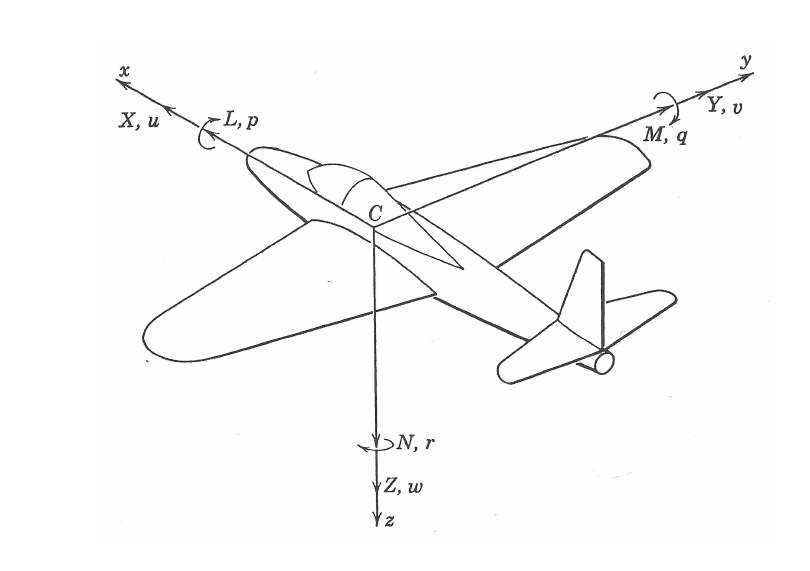
\includegraphics[width=\linewidth]{figs/axis1.png}
  \caption{Coordinates system and relevant variables.}
  \label{fig:coords1}
\end{figure}

Where:


\begin{itemize}

\item $x$, $y$, and $z$ are the coordinates, with the origin in the vehicle's center of mass.
\item $u$, $v$, and $w$ are the linear velocities in each of the $x$, $y$, and $z$ coordinates, respectively.
\item $X$, $Y$, and $Z$ are the components of the aerodynamic force in each of the $x$, $y$, and $z$ coordinates, respectively.
\item $p$, $q$, and $r$ are the linear velocities in each of the $x$, $y$, and $z$ coordinates, respectively.
\item $u$, $v$, and $w$ are the linear velocities in each of the $x$, $y$, and $z$ coordinates, respectively.
\item  Although not indicated in the figure, the variables $\phi$, $\theta$, $\psi$ represent the angular rotations,
relative to the equilibrium state, about the x, y, and z axes, respectively. Thus, $p=\dot{\phi}$, $q = \dot{theta}$
and $r = \dot{\psi}$ where the dots represent time derivatives.

$\phi$, $\theta$, and $\psi$ can also be referred, respectively, as \textit{roll}, \textit{pitch}, and \textit{yaw}.

\end{itemize}

\section{VTOL Mechanics}

When in VTOL mode, the coordinate system used is similar to that in a conventional multirotor, with $Z$ pointing up parallel the motors axis, and $X$ going throw the fuselage, pointing away from the belly of the aircraft.

The mechanics involved in vertical take-offs and landings is slightly different. The lift generated becomes meaningless, no more than a slight perturbation to the system. The generated thrust becomes directly responsible for vertical motion and roll control, while the control surfaces can redirect the airflow allowing control of yaw and pitch.

The approximate model, as seen on \todo{citation needed} is :

\todo{formula needed}


\section{XFLR5}

XFLR5 is an analysis tool for airfoils, wings and planes operating at low Reynolds Numbers. It includes:
\begin{itemize}

\item XFoil's Direct and Inverse analysis capabilities;
\item Wing design and analysis capabilities based on the Lifting Line Theory, on the Vortex Lattice Method, and on a 3D Panel Method.

This tools enables the iterative design and analysis of multiple aircraft configurations.

\todo{elaborar aqui}

\end{itemize}


\section{Design}

The chosen design is the one of a flying wing, a fuselage-less made of a wing, propulsion system, and control surfaces. The reasons are because of a simpler and sturdier mechanical structure, besides the possibility of the VTOL configuration

\subsection{Preliminar Design}

As a starting point, a wing with a central hub and 2 semi-wings ending in symmetrical winglets was designed. The ZAGI12 airfoil was chosen due to it's good soaring capabilities and low stall speed \todo{citation needed}.

With the airfoil chosen, It's characteristics were calculated with the aid of XFOIL, an airfoil analysis tool built into XFLR5.

\begin{figure}
\centering
  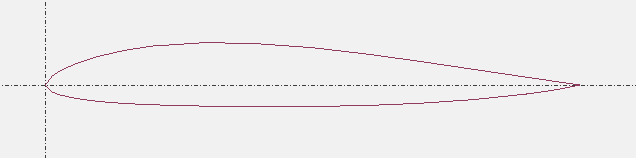
\includegraphics[width=\linewidth]{figs/zagi12.png}
  \caption{Zagi 12 airfoil.}
  \label{fig:zagi12}
\end{figure}


These characteristics plots can be seen on figure \ref{fig:zagi12polares}.
%

It can be noted that the point with the highest Cl/Cd ratio, the theoretical point with better lift to drag ratio, and therefore best gliding performance. It's also notable that the airfoils moment "pulls" it into this better Cl/Cd ratio, allowing the aircraft to fly into this ideal condition without deflection of the control surfaces


\begin{figure}
\centering
  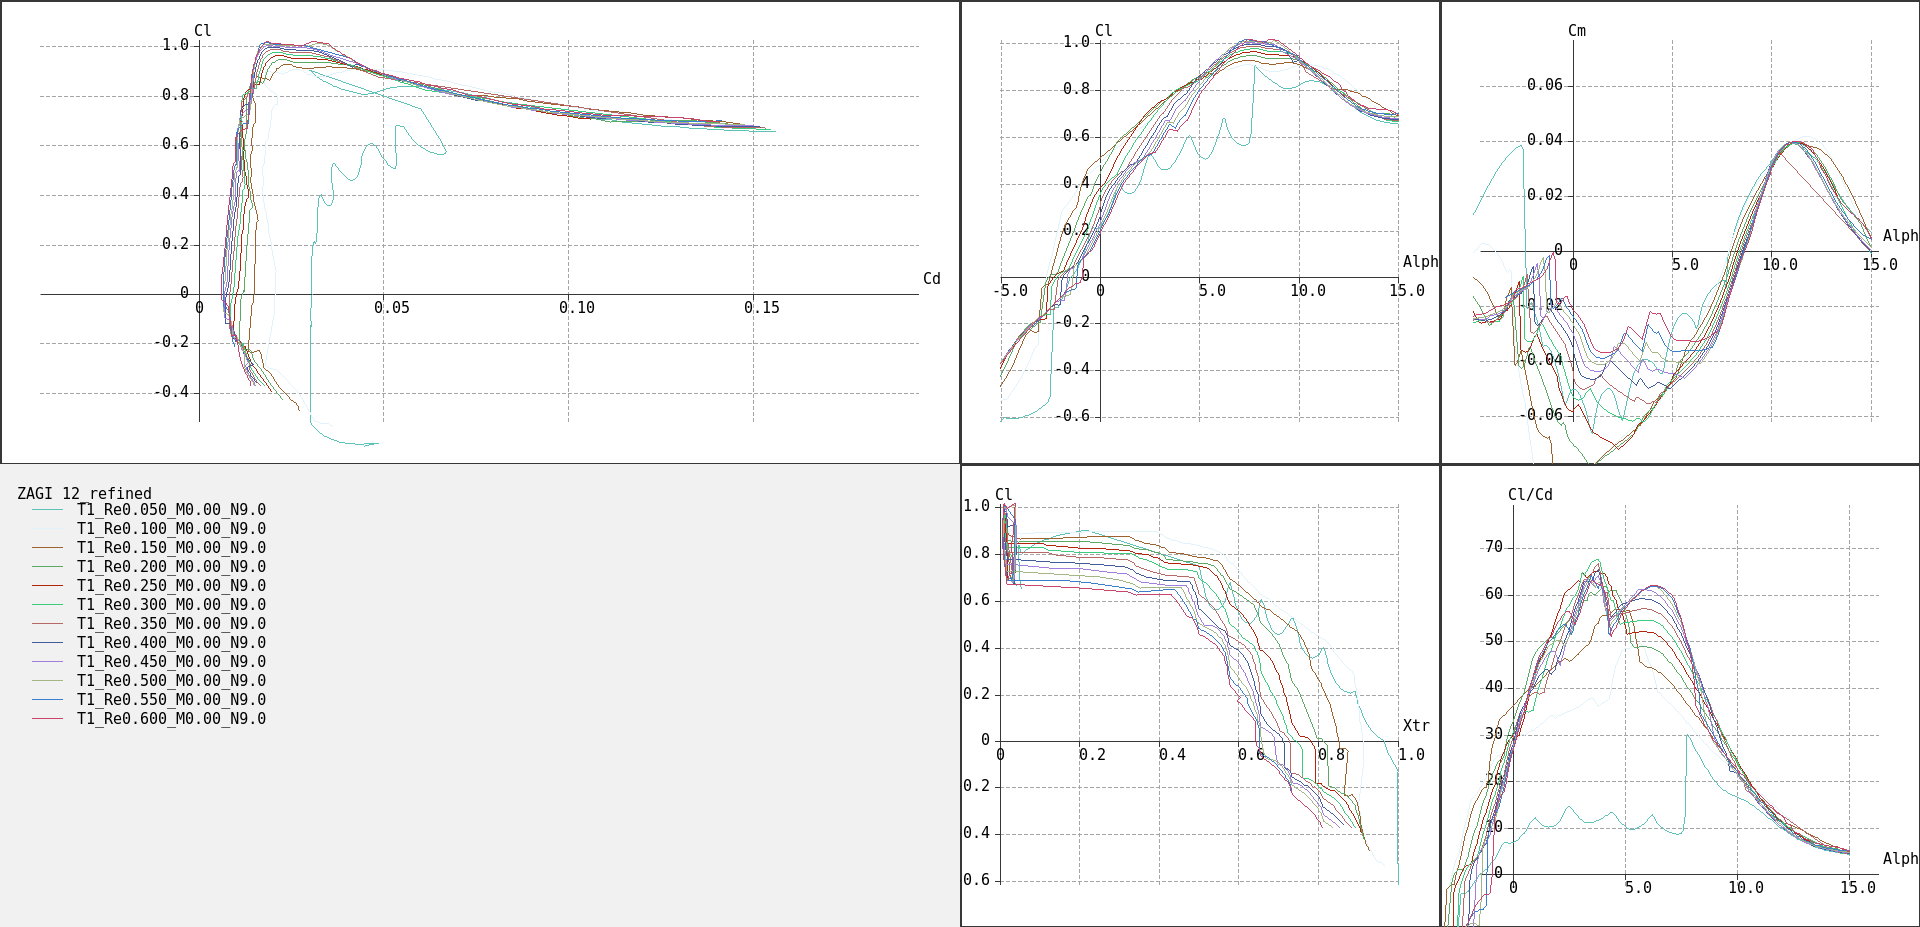
\includegraphics[width=\linewidth]{figs/polares.png}
  \caption{Zagi 12 characteristics}
  \label{fig:zagi12polares}
\end{figure}

With that data, the main body was conceived, as seen in the figure \ref{fig:preliminar}. With this CAD tool we can then analyze the performance of the aircraft as a whole. This gives us the same data as the airfoils', but for the whole craft, as seen in figure \ref{fig:craftpolar}.

Some data can be inferred from these graphs. From \ref{fig:zagi12polares} it can be seen that the highest $C_l$, or Lift Coefficient, is obtained around $\alpha = 8\deg$, which, possibly by design of the airfoil, is also the zone with a higher $C_l/C_d$, or \textit{lift-to-drag ratio} maximizing the gliding distance. It's also notable tat the $C_m  \times \alpha$ plot crosses 0 around the the same $8\deg$, meaning the profile is generally trying to point at that angle.

\begin{figure}
\centering
  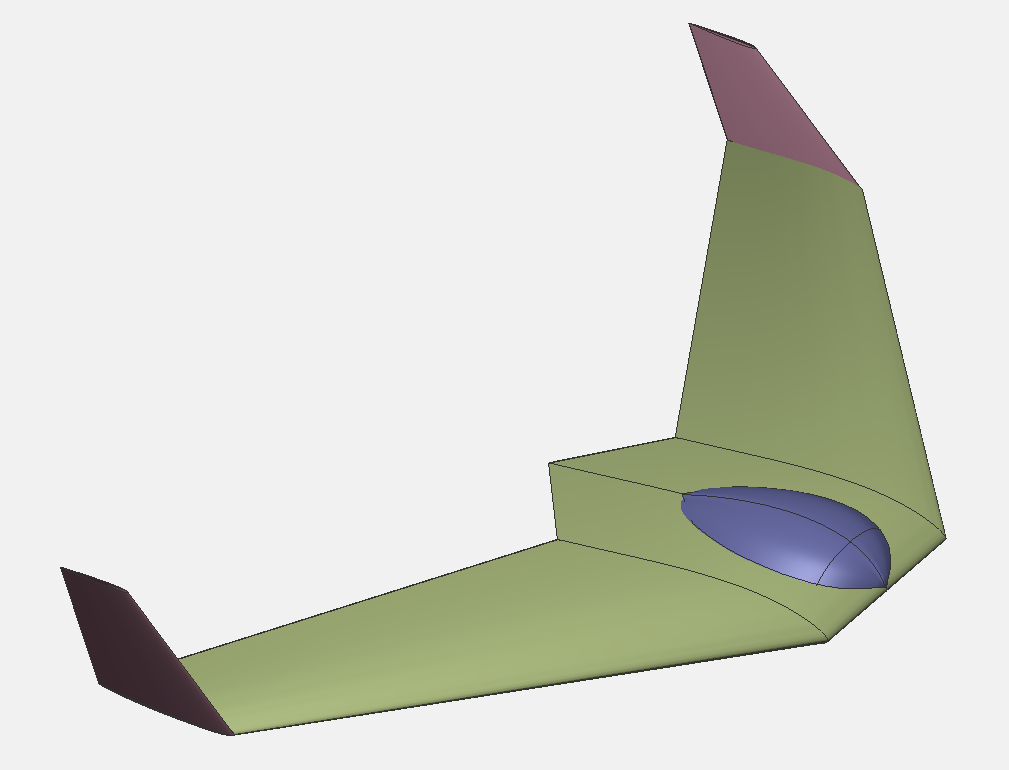
\includegraphics[width=\linewidth]{figs/preliminar.png}
  \caption{First concept of the aircraft.}
  \label{fig:preliminar}
\end{figure}


From \ref{fig:craftpolar}, 	

\begin{figure}
\centering
  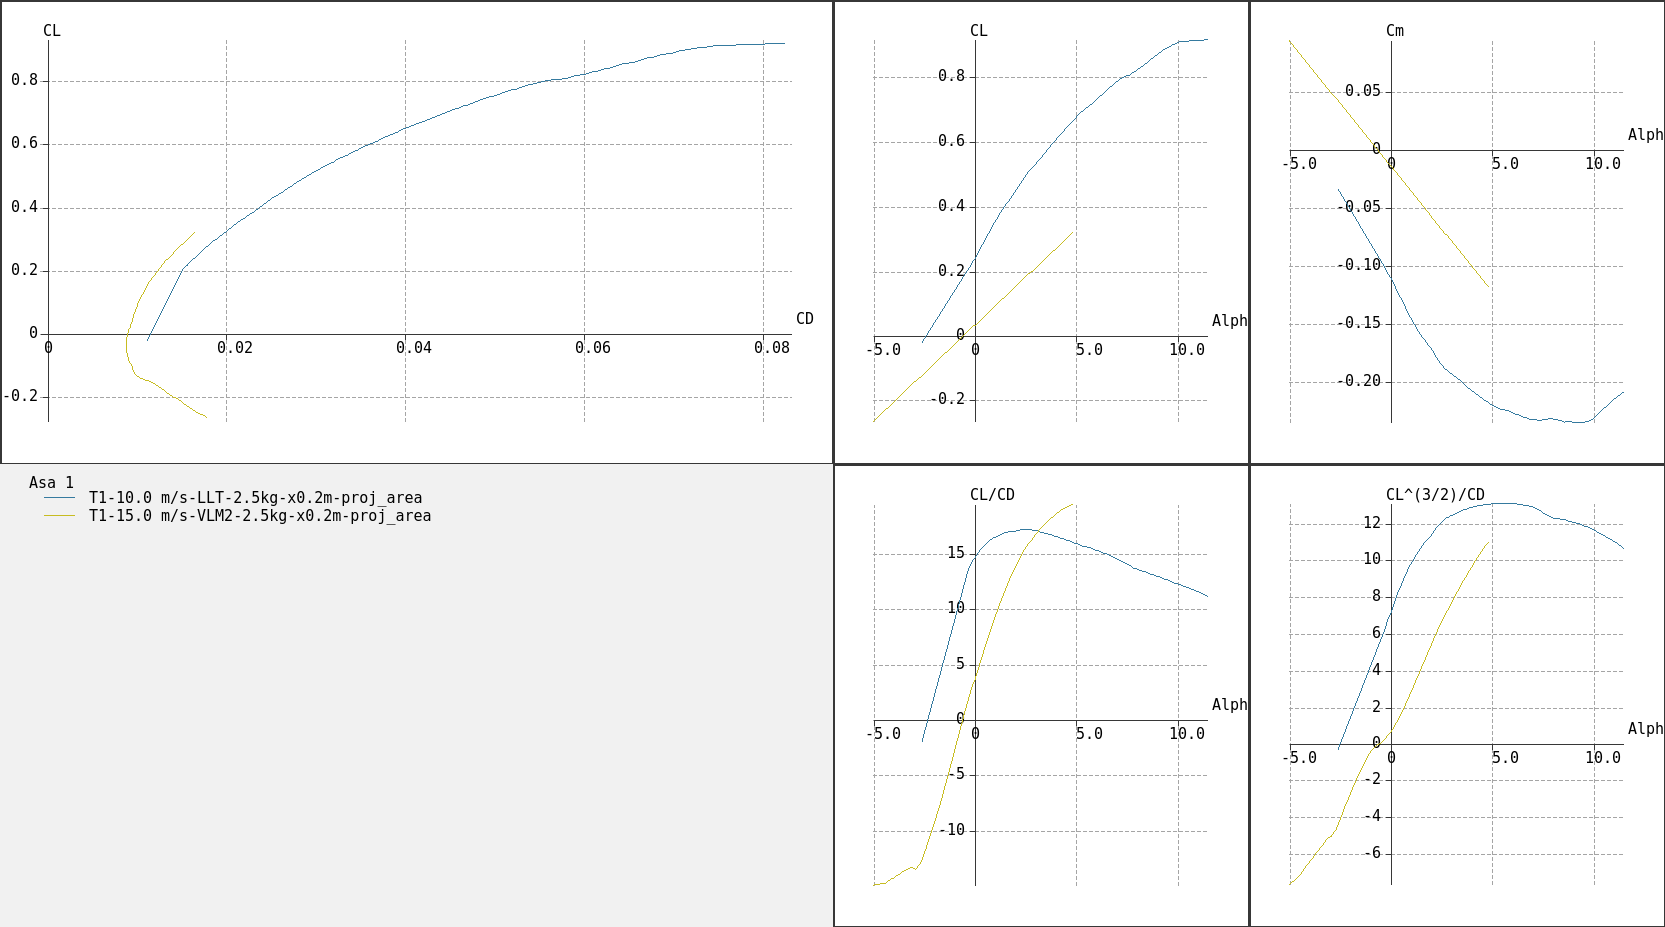
\includegraphics[width=\linewidth]{figs/craftpolar.png}
  \caption{Flight characteristics of the preliminary aircraft design.}
  \label{fig:craftpolar}
\end{figure}


\subsection{Final Design}

Due to building issues and the desire to maximize both effective payload and flight autonomy, the design was simplified, extending the chord back on the beginning of the wings, as seem on figure \ref{fig:final}
	

\begin{figure}
\centering
  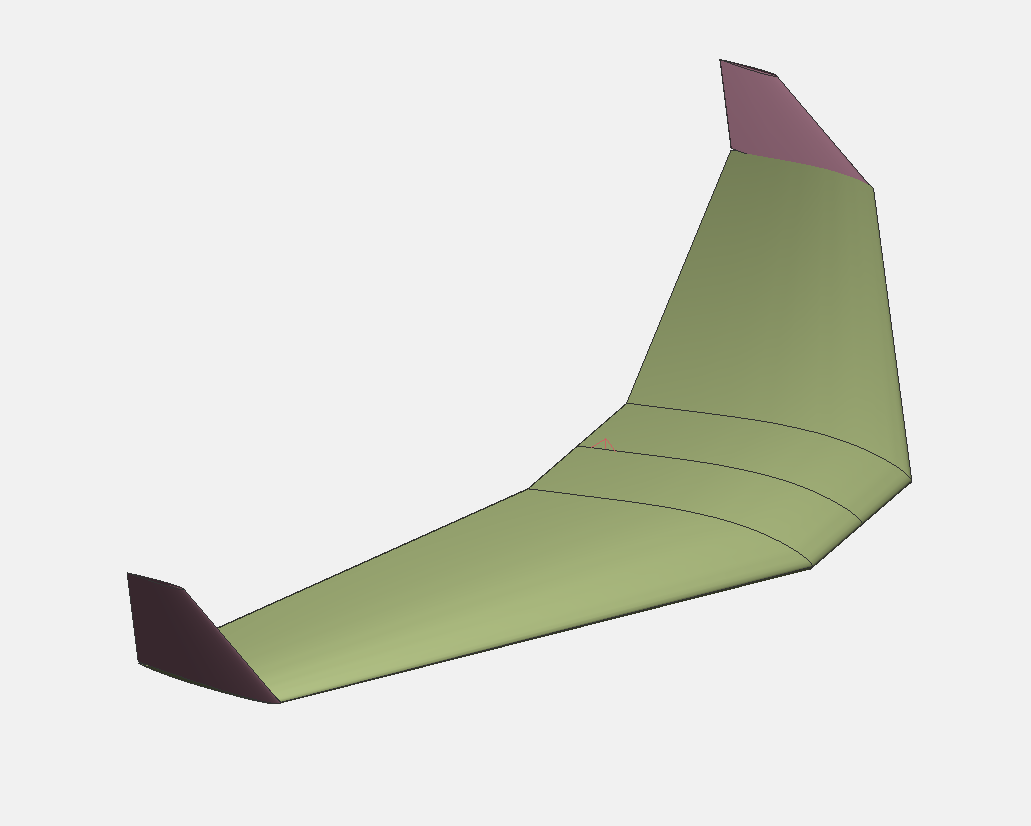
\includegraphics[width=\linewidth]{figs/final.png}
  \caption{Final design of the aircraft, on XFLR5.}
  \label{fig:final}
\end{figure}

\begin{figure}
\centering
  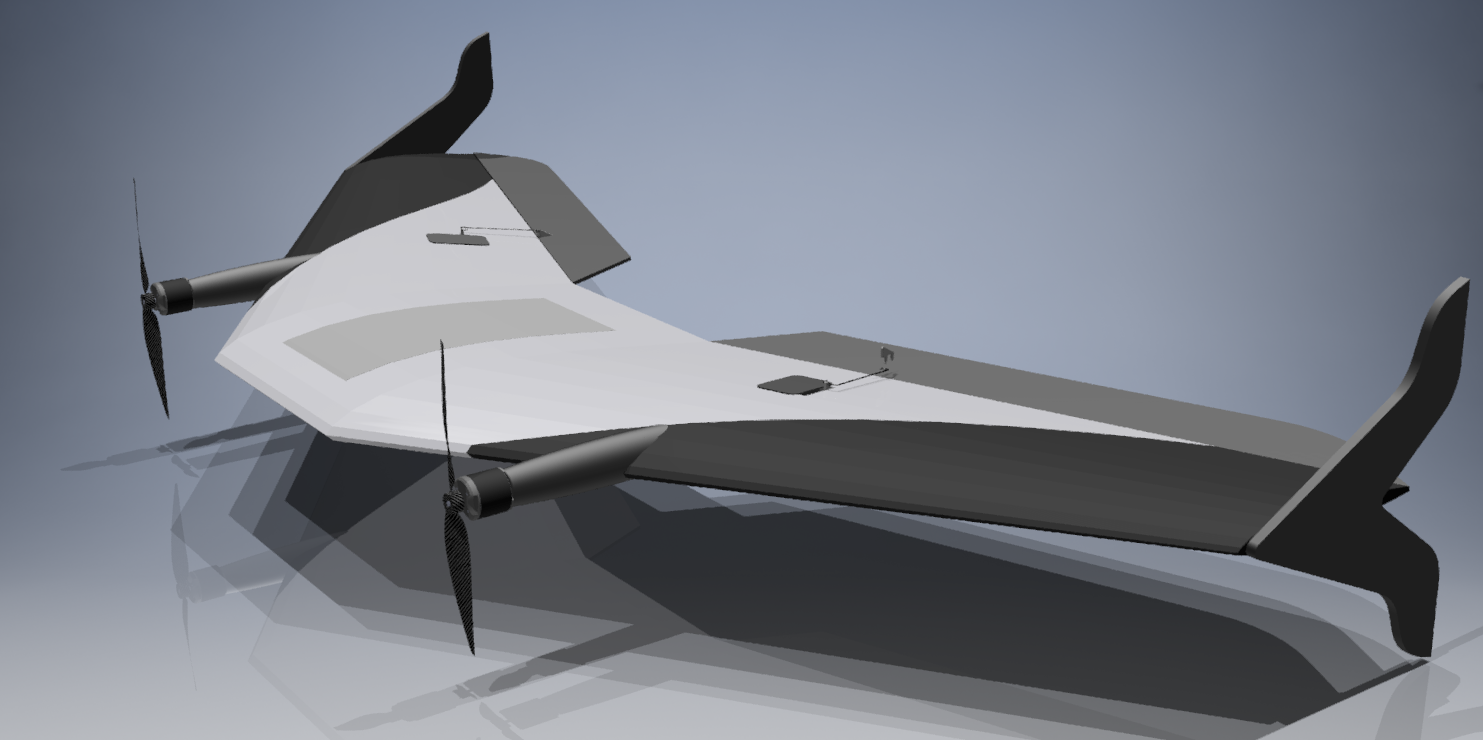
\includegraphics[width=\linewidth]{figs/finalrender.png}
  \caption{Final design of the aircraft.}
  \label{fig:finalrender}
\end{figure}

\begin{figure}
\centering
  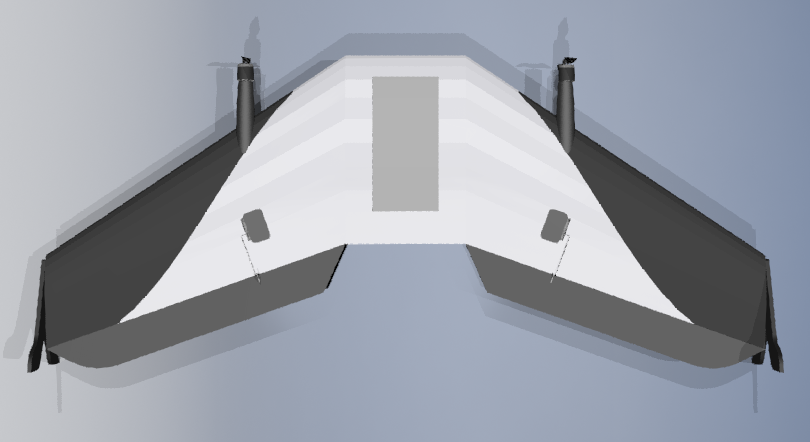
\includegraphics[width=\linewidth]{figs/finalrendertop.png}
  \caption{Final design of the aircraft, top view.}
  \label{fig:finalrendertop}
\end{figure}


%%%%%%%%%%%%%%%